\section{實驗與實體驗證}

\subsection{機器人定位}

此專題以室內高精準度定位為目標,配合深度相機之影像辨識與物體深度,找到目標物之位置並標記。

\paragraph{定位準確度測試}

本專題之定位裝置使用Ultra-wideband超寬頻通訊天線,為提供目標物位置之量測精準度,設計此定位精準度測試。鋪設5*5巧拼,量測各點之UWB定位座標,比較Ground Truth,進行多次量測後計算方均根值作為誤差數據,實驗結果如表
\ref{table:localization_error}所示。將結果之數據量化後標示於地圖上如圖\ref{figure:localization_result}所示。

\begin{table}[h]
	\centering
	\begin{tabular}{| c| c| c|}
		\hline
		Ground Truth X (m) & Ground Truth Y (mm) & 定位誤差 (mm) \\ 
		\hline
		300 & 300 & 68.43 \\ 
		\hline
		1500  & 300 & 117.58 \\ 
		\hline 
		2700  & 300 & 64.69 \\ 
		\hline 
		2700  & 1500 & 195.94 \\ 
		\hline 
		2700  & 2700 & 220.11 \\ 
		\hline 
		1500  & 2700 & 200.33 \\ 
		\hline 
		300  & 2700 & 56.93 \\ 
		\hline 
		300  & 1500 & 27.56 \\ 
		\hline 
		1500  & 1500 & 50.39 \\ 
		\hline 
	\end{tabular}
	\caption{定位測試}
	\label{table:localization_error}
\end{table} 

\begin{figure}[bht]
	\centering
	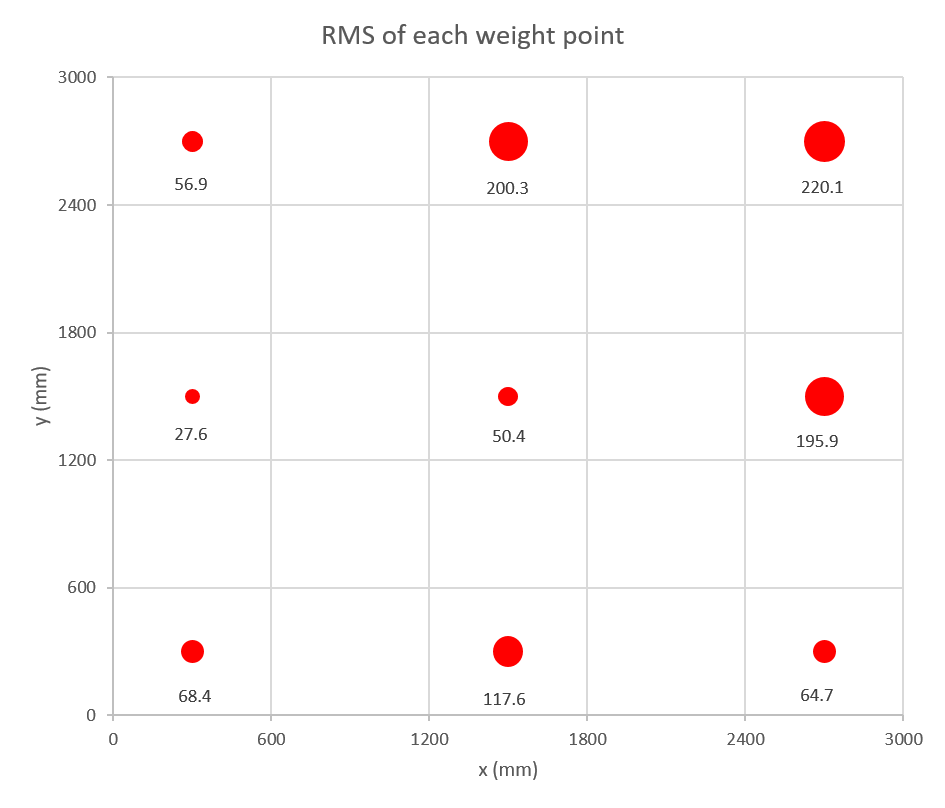
\includegraphics[height=!,width=\linewidth,keepaspectratio=true]
	{images/uwb_bench.png}
	\caption{以UWB定位之誤差量測實驗結果}
	\label{figure:localization_result}
\end{figure}

\paragraph{定位測試影片} 

本專題利用UWB之定位結果經過移動限制過濾器後繪製出行進軌跡,測試影片連結如下:

\begin{itemize}

\item
載具利用遙控行進場地一圈並繪製出軌跡圖
\url{<Put URL Here>}

\item
避障實驗一(靜態障礙物): 
\url{https://youtu.be/ve4Mln4D1xo}

\end{itemize}


\subsection{影像辨識}

本專題比較目標物於各版本SSD運算量及FPS後,如\ref{table:fps_compare},選擇FPS較高且運算量較低的MobileNet-V1 SSD,使用Jetson Nano執行Model。
並配合深度相機於標記目標物後,將bounding box之中點位置利用矩陣投影的方式找出目標物與相機之距離,如\ref{figure:vision}。

由如\ref{figure:evaluation}可以發現到Duck的Average Precision會比其他的還要來的低只有0.58,明顯的看出MobileNet-SSD對於小物品的偵測相對於其他model如yolo較不理想。


\begin{table}[h]
	\centering
	\begin{tabular}{| c| c| c|}
		\hline
		Frame Rate (FPS) & desktop 1080 & Jetson Nano \\ 
		\hline
		SSD & 36 & 1.5 \\ 
		\hline
		MobileNet-V1 SSD  & 90-100 & 16.5 \\ 
		\hline 
		MobileNet-V2 SSD & 78-80 & 12 \\ 
 
		\hline 
	\end{tabular}
	\caption{各版本FPS比較}
	\label{table:fps_compare}
\end{table} 

\begin{figure}[t]
	\centering
	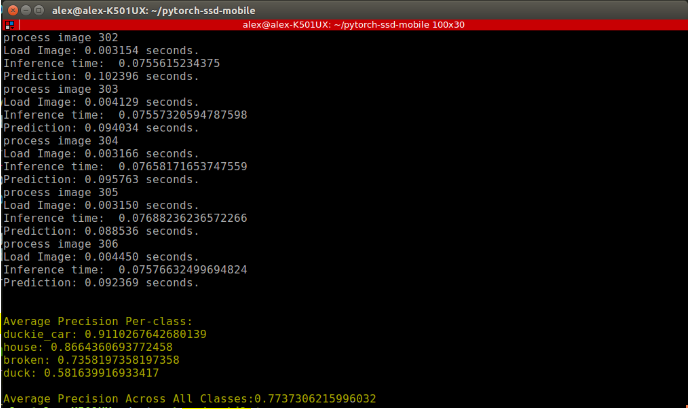
\includegraphics[height=!,width=\linewidth,keepaspectratio=true]
	{images/evaluation.png}
	\caption{MobileNet-V1 SSD evaluation}
	\label{figure:evaluation}
\end{figure}

\begin{figure}[h]
	\centering
	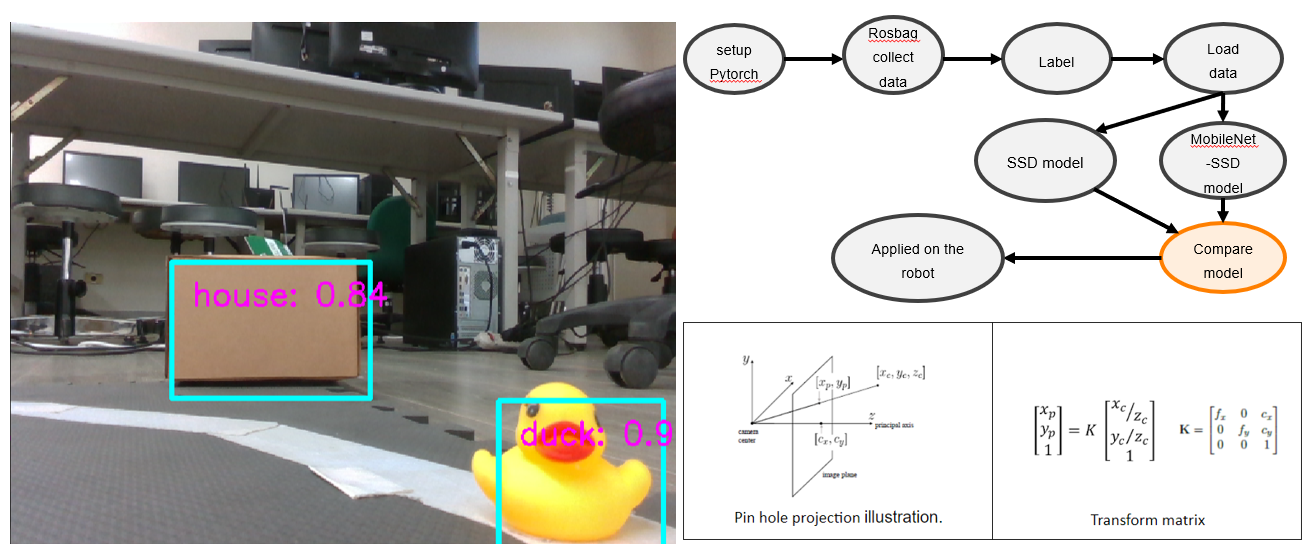
\includegraphics[height=!,width=\linewidth,keepaspectratio=true]
	{images/vision.png}
	\caption{預測目標物之實驗步驟及相對距離投影矩陣}
	\label{figure:vision}
\end{figure}


